\chapter{Protoype}
\label{prototype}

\section{The Host Platform}
The prototype system is implemented in Clojure \cite{hickey}, a language in the Lisp family which runs on the Java Virtual Machine \cite{gosling}. Clojure also fills the role of the host kernel language. Some characteristics of Clojure that make it a good choice include:
\begin{enumerate}
\item Similar notion of a kernel language. The prototype simply adopts (a subset of) the special forms of Clojure as its kernel language.
\item Functional orientation. Clojure is a non-pure functional language; it allows side-effects but (in contrast to most Lisps) all of its bindings and data structures are immutable. %Destructive assignment is supported only for special \emp{reference} objects which enforce certain semantics (and which do not play any real role in this system). This approach fits quite well with the idea of transformation of immutable trees, and in fact inspired many ideas such as the approach to tree reduction.
\item Compilation service available at runtime. The Clojure compiler is part of the runtime stack, so once a program is reduced to the kernel language, it can be evaluated (compiled) and executed immediately.
\item Access to the Java platform. The prototype takes advantage of Java's GUI toolkit for rendering and editing.
%\item Compiles to Java bytecode, and allows direct access to the platform's objects when needed. For example, nodes are represented as instances of a class at the JVM level, which gives excellent performance with no representational overhead. It's some kind of triumph of compiler technology that a program in this system can achieve performance on par with raw C code. \todo{need to prove that?}
\end{enumerate}

A handful of node representations are implemented for different purposes. First, a Lisp-style ADT for nodes is implemented as a series of functions \clojure{make-node}, \clojure{node?}, \clojure{node-type}, etc., which allow Clojure programs to construct and manipulate nodes, independent of the concrete representation. The prototype uses only these functions to work with nodes.

The implementation of the node ADT uses Clojure's \clojure{deftype} construct to represent nodes as instances of a \clojure{nodetype} class at the JVM level. This reduces the overhead for simple nodes to the minimum. Map- and sequence-valued nodes use Clojure's built-in persistent hash map and persistent vector (array-mapped trie [?]) data structures to store their children.

The \clojure{make-node} function provides a convenient serialized form for nodes: s-expressions. A \clojure{print-node} function turns a node object back into text which can be read and evaluated to re-constitute the node.


\section{The Host Language}
\label{host}
The host language is composed of a kernel based on the primitive constructs and values of Clojure together with a core language built via syntax extension on top of the kernel language.

The kernel language, shown in Figure \ref{fig-kernel}, consists of six kinds of primitive values, six node types corresponding to Clojure's special forms, two nodes for quotation, and a node for making external references to the platform.

The kernel language is somewhat simplified relative to the complete list of Clojure's special forms. A few forms which are not currently used are left out, and several of the nodes are somewhat less flexible in form than the corresponding Clojure syntax.

\begin{figure}
  \todo{fix columns? clean up primitives with some syntax}
  
%  \fbox{
  \begin{minipage}[t]{0.48\linewidth}
  \vspace{0pt}  % align to top
  \begin{center}
  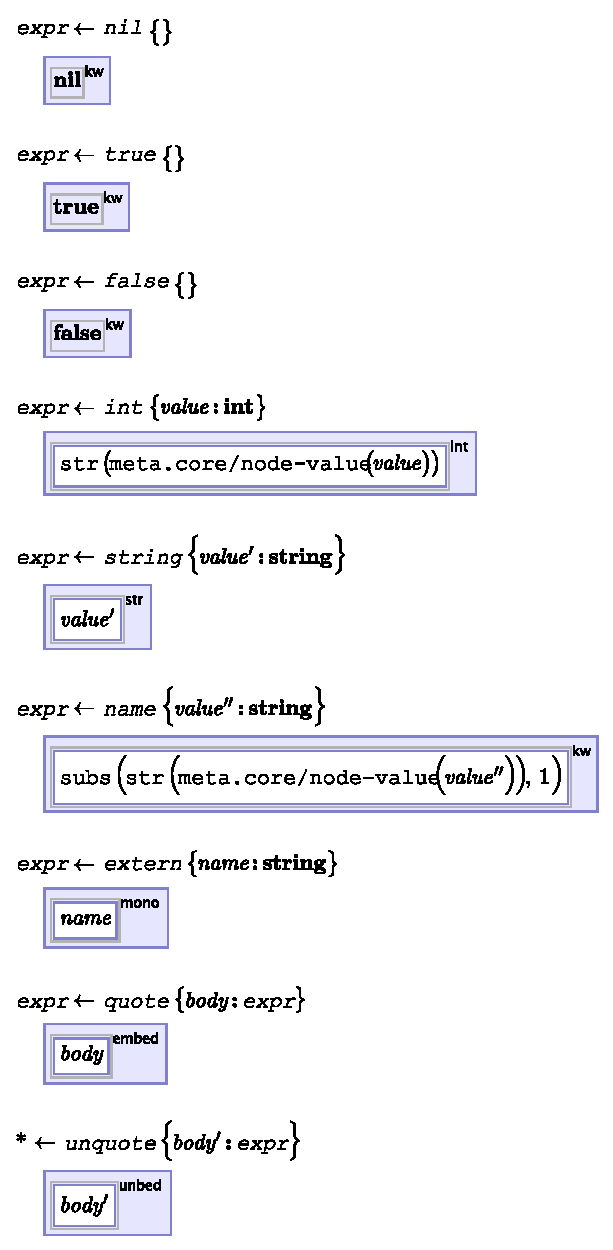
\includegraphics[scale=0.65]{src/image/kernel1.pdf}
  \end{center}
  \end{minipage}
%  }
%  \hfill
%  \fbox{
  \begin{minipage}[t]{0.48\linewidth}
  \vspace{0pt}  % align to top
  \begin{center}
  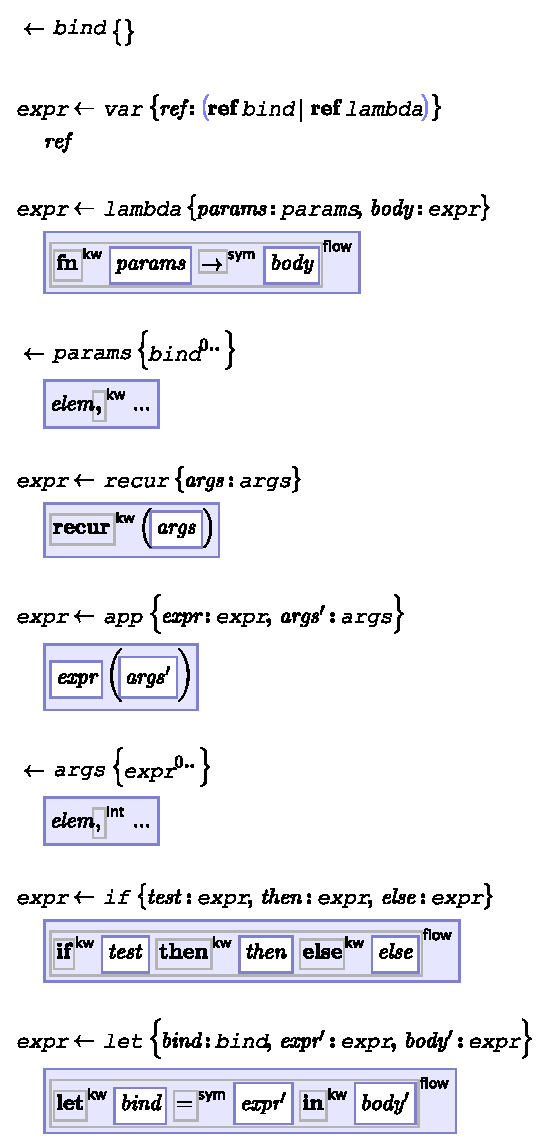
\includegraphics[scale=0.65]{src/image/kernel2.pdf}
  \end{center}
  \end{minipage}
%  }
  
%(\keyword{loop}, \keyword{recur})

  \caption{\label{fig-kernel} Grammar for the host kernel language.}
\end{figure}

\subsection{Kernel Language Semantics}
The primitive values of the kernel language are the singular values \keyword{nil}, \keyword{true}, and \keyword{false}, plus integers, strings, and names.

A \keyword{lambda} node introduces a function taking a fixed number of arguments. A \keyword{params} node always represents the parameters of a function, and can appear only as the \keyword{params} attribute of a \keyword{lambda} node. Each parameter is a \keyword{bind} node, discussed later. A lambda node is ``bound'' within its body, supporting simple recursive calls. \keyword{recur} is a non-stack-consuming recursive call, and must appear in tail position.

$n$-ary functions are included in the kernel language as they are in Clojure to allow a simple mapping to Java methods. The kernel language does not support Clojure's variable-arity functions.

\keyword{app} is (call-by-value) function application. An \keyword{exprList} node contains expressions to be evaluated from left to right.

\keyword{let} evaluates an expression, binds a name to the resulting value and then evaluates its body with that binding in scope. \Meta\ provides only a single-binding \emp{let} form, and no \emp{letrec} (Clojure provides a separate \clojure{letfn}, which is not currently available in \Meta). 

A \keyword{var} node is a reference to the value bound by the parameter of a lambda, by the lambda itself, or by a let expression. 

Simple conditionals are provided by \keyword{if}.

Variables are lexically-scoped, and lambdas capture all bindings in scope at their point of declaration.

An \keyword{extern} node refers to a variable at the Clojure level. This allows any function or value defined by the Clojure platform or \Meta\ runtime to be accessed. Use of these external facilities is minimized in order to make the core language as self-contained as possible. 

\keyword{quote} and \keyword{unquote} are handled by the meta-compiler as described below.

\subsection{Meta-compilation}
Given a program in the kernel language, a function \clojure{meta-compile} translates the nodes to Clojure s-expressions in a mostly straight-forward way, due to the close correspondence between kernel nodes and Clojure's special forms. Only a few types of nodes need special consideration. %Then Clojure's \clojure{eval} function is invoked, and the program is compiled to Java bytecode, loaded into the JVM, and executed. Because the kernel language maps so closely to Clojure's forms, the meta-compilation process is mostly trivial.

%Each kernel language node corresponds precisely to a Clojure special form or value, without any additional interpretation. Furthermore the structure of a Clojure program after reading matches the structure of the kernel program precisely: a Clojure program is a tree made from lists where the first element of each list is a symbol which names a special form. For example, the list produced by the reader for the string \clojure{"(+ 1 (* 2 3))"} has exactly the same overall shape as the corresponding kernel language program, with lists replaced by \keyword{app} nodes, and the simple names \clojure{*} and \clojure{+} wrapped in \keyword{extern} nodes. \todo{include a picture of the nodes version? How to do that without going into presentation issues? Can I avoid having tons of pictures of trees?}

A \keyword{bind} node is reduced to a symbol, and a \keyword{var} node to the symbol of the corresponding binding. The problem of producing suitable names and avoiding conflicts is easily solved due to the uniqueness of labels in the \Meta\ program. The meta-compiler simply generates a new name for each label and uses that name for both \keyword{bind} and \keyword{var} nodes.

When the meta-compiler encounters a \keyword{quote} node, it enters a separate mode where instead of translating kernel language nodes to s-expressions, it instead translates nodes (potentially in any language) to s-expressions that construct the quoted nodes. When an \keyword{unquote} node is encountered, the meta-compiler reduces the contents in the normal way, and then inserts the resulting value into the expression building the quoted node. Quotations may be nested more than one level deep, so the reduction keeps track of the current level and only resumes ordinary translation when the level reaches zero.

\temp{make the point about how this addresses hygiene? or is that somewhere else?}

Once a kernel language program has been meta-compiled, the standard Clojure function \clojure{eval} is invoked, which compiles the expression to Java bytecode, loads it into the running JVM, invokes it, and returns the result as a Clojure/Java value. %When necessary a function is available to ``wrap'' that value in (kernel language) nodes which represent the same value. This \emp{unread} mechanism will be discussed later. \todo{Will it? Come back to these implementation details later or not?}


%\subsection{Limitations}
%When nodes are translated to s-expressions, all information about the origin of the code is lost. This means that exceptions and stack traces cannot identify the source locations.


%
% Rendering :expr:
%
\section{Rendering the Expression Language}

\subsection{The \keyword{view} Language}
\label{view}
To fulfill the promise of the language-independent \keyword{expr} language, its logical nodes need to be reduced to something that can be rendered on screen. This is accomplished via reduction to a lower-level \keyword{view} language. The view language is modeled on the concepts of \TeX's math mode\cite{tex-math}, and some of the algorithms of \TeX\ are used to lay out nodes and construct glyphs. This is a common approach\cite{mathml}.

The view language is consumed by a \emp{renderer} written in Clojure using the graphics primitives of Java2D\cite{java2d}. The renderer recursively inspects the \keyword{tree}, calculating node sizes and layout, and then actually drawing nodes to a provided context.
The renderer also provides hit-testing for nodes, identifying a list of \keyword{view} nodes which enclose a given point. It also draws visual indicators of selected nodes and nodes with errors, which are identified by id.

%\begin{figure}
%\todo{capture the real thing}

%\keyword{chars}

%\keyword{thinspace}, \keyword{mediumspace}, \keyword{thickspace}, \keyword{quad}

%\keyword{sequence}, \keyword{section}

%\keyword{scripted}

%\keyword{over}, \keyword{radical}

%\keyword{delimited}

%\keyword{border}

%\keyword{rgb}, \keyword{gray}, (\keyword{color})

%\caption{\label{fig-view} Grammar for the low-level \keyword{view} language.}
%\end{figure}

The nodes of the \keyword{view} language parallel the nodes of \keyword{expr} (see Figure \ref{fig-view}), but logical nodes have been reduced to a concrete representation. For example, for the various atom types, there's a single \keyword{chars} node, which contains a string and font. \keyword{sequence} is used to represent all horizontal sequences without any implied spacing. \keyword{section} is a simple vertical arrangement of left-aligned nodes.

The \keyword{scripted}, \keyword{over}, \keyword{radical},and \keyword{delimited} nodes were described earlier. \keyword{border} draws its content with a background color, surrounded by a rectangular border with a configurable weight.

Nodes which draw glyphs can have a \keyword{color} attribute, which causes the single node to be drawn with a different foreground color.

For layout purposes, the renderer calculates a size for each node, consisting of width, height, and baseline height (which may be undefined). A baseline is calculated for each \keyword{chars} node based on its font, and certain other nodes calculate a baseline based on their contents. \keyword{sequence} nodes' children are laid out so that nodes with baseline heights are aligned to a mutual baseline, and nodes without baseline heights are aligned to their vertical center (and the overall vertical center of all baseline-aligned siblings). This is sufficient to get simple expressions to render well, but the current algorithm lacks \TeX's second alignment step (the \emp{axis}), which would be needed to get certain sub-expressions such as fractions to be properly aligned.
 
\keyword{radical} and \keyword{delimited} nodes are laid out by first sizing the content node, then selecting the appropriate glyph(s) from a list of variously-sized alternatives, and finally calculating sizes and positions based on the selected glyph. \TeX's fonts are used for these glyphs, as well as for most symbols reduced from \keyword{expr/symbol}. 


\subsection{The Renderer}

The renderer makes several passes over the tree to draw different layers. The first pass draws only \keyword{border} nodes, which therefore appear ``behind'' all other elements. The nodes are drawn in pre-order, so that parent borders and their background fill are drawn behind any child borders. On the second pass, an indicator of the selected node is drawn, so that it will appear above the border rects, but behind the actual content. The final pass renders all non-border nodes. \todo{error indicator?} 

The renderer is written in a simple functional style, freely traversing the node tree as much as necessary. However because size calculations are relatively expensive, this na\"{\i}ve \todo{wc?} approach initially led to poor performance of drawing and hit-testing (on the order of 2-500ms to render a small program). This was easily improved by simply memo-izing two kinds of functions. The function that calculates the size of a text glyph given the characters and font is simply memo-ized, so that no more than one call is ever made for each unique glyph. The functions that calculate size and position for each node are also cached, but only for the duration of a single rendering pass. That way the renderer performs well (10-20ms) despite being written in the most direct way, making no attempt to reduce redundant calculations. Clojure's functional nature and macro facility made it easy to implement this algorithmic change ``after the fact,'' without requiring the renderer to be re-written.

The renderer currently violates good functional programming style by performing the actual drawing via side-effecting operations during the traversal of the node tree. In hindsight, it would have been better t0 have the traversal yield a list of drawing commands to be executed later. For instance the layering of different kinds of visual elements could have been handled explicitly, rather than as a side-effect of traversal order. If the renderer was implemented as a reduction to an even lower-level language consisting of nodes corresponding directly to the drawing operations of Java2D, it would nicely unify the layers of the system.


\subsection{Reducing \keyword{expr} to \keyword{view}}
The reduction from \keyword{expr} to \keyword{view} is the most complex in \Meta, because it involves some non-local information. It is written by hand using an enhanced reduction algorithm which keeps track of a pair of values at each node: \emp{display mode} and \emp{meta-level}.

The mode, a concept from \TeX, identifies the depth of nesting of expressions, and controls the selection of font sizes for atoms. There are four modes, \textit{Display} ($D$), \textit{Text} ($T$), \textit{Script} ($S$), and \textit{Scriptscript} ($SS$). By default, the mode of the root node is $T$, and the mode is decreased (roughly in sequence) whenever notational convention dictates that subexpressions should be typeset in a smaller font. When reducing an atom, the atom type and mode are used to look up the appropriate font. The handling of modes follows \TeX's algorithm in most cases, but deviates from it when necessary for consistency. For example, typographical convention dictates that addition expressions in the smaller modes should be set without spaces, but that would clash with \Meta's handling of parentheses, so \Meta\ sets these expressions with proportionately smaller spaces.

\begin{figure}[h]
\begin{center}
\todo{capture something real}
\end{center}

$$
\mathrm{D:} \quad
a + b^2 + x^{c_1}
 - { x^{i+1} \over y }
 + { 1 \over { 1 \over R_1 }
 + { 1 \over R_2} }
 - \left({ 1 \over R_1 } + { 1 \over R_2}\right)^{-1}
$$

$$
\mathrm{T:} \quad
\textstyle
a + b^2 + x^{c_1}
 - { x^{i+1} \over y }
 + { 1 \over { 1 \over R_1 }
 + { 1 \over R_2} }
 - \left({ 1 \over R_1 } + { 1 \over R_2}\right)^{-1}
$$
\caption{\label{fig-modes} Program fragment with multiple modes.}
\end{figure}

As the example in Figure \ref{fig-modes} shows, the smaller modes quickly become hard to read for anything but very simple expressions (especially on relatively low-resolution displays), so wise language designers (and programmers) will use them sparingly. The \TeX book\cite{knuth} gives much good advice about how to use them effectively. The most clear application of the smaller modes in ordinary programs is for decorating variable names with small integer subscripts and primes.

The meta-level is a non-negative integer indicating the level of nesting of the current node. It begins at zero and is incremented whenever an \keyword{embed} node is encountered and decremented on \keyword{disembed}. The \keyword{embed} node itself is reduced to a \keyword{border} which draws a light-colored background behind the embedded nodes, and a darker border of the same hue. An \keyword{disembed} node becomes a border with the hue of the lower level and the background of the outer level, making a visual connection between the outer and nested nodes that are at the same level. A fixed series of colors is used that can unambiguously indicate nesting of up to a half-dozen levels. Examples appear in figures \ref{fig-flarp} and \ref{fig-zeb}.

To compute the mode and meta-level at each node, the reduction function is extended to take the two values as additional parameters, and to return the pair of values along with the reduced node each time it is invoked. As the tree is visited, the values that were computed for a given node are passed to the reduction for its children. This allows the reduction function to compute values based on the shape of the tree, which would otherwise be impossible due to the lack of any reference from a sub-tree to its parent node. Effectively, the ``inherited'' value allows the reduction function to accumulate some information about the otherwise inaccessible ancestors. This simple extension is sufficient for this reduction (the most complicated yet encountered), and it does mean that this reduction could not be implemented in a grammar as almost all other reductions in \Meta\ are. It would be possible to define a grammar language that would support this kind of reduction, perhaps by adopting some of the semantics of attribute grammars\ref{attribute-grammar}.


\subsection{Meta-reduction of \keyword{expr}}
When editing regular programs, the \keyword{expr} language is meant to be invisible. When editing a grammar, the \keyword{expr} nodes of each presentation reduction are the subject at hand, so it's necessary for understanding to make them visible. To accomplish this, another hand-written reduction is used when editing grammars. This reduction decorates each node with a visual indication of its type, location, and size. This reduction is somewhat idiosyncratic in that it never actually replaces a node, but rather it inserts additional nodes (super-scripted \keyword{border} nodes), which surround the original nodes. Also, this reduction needs to be restricted to operate only on \keyword{expr} nodes of the original program, and not any nodes that might have been introduced by a reduction that was applied earlier. The reduction function is wrapped in a higher-order function that uses the reduction value to track which nodes remain to be reduced.

The result can be seen in any of the examples of presentation reductions presented earlier. The idea of using a higher-order function (combinator) to assemble multiple simple reductions into something more complex came up again and again in building the prototype.


\subsection{Generalized reduction}
Another useful reduction is one that is able to reduce any arbitrary node, imposing no restrictions whatsoever on the type or value of the node. This reduction can be used to show the internal structure of a node, disregarding the presentation reduction, as in the \Meta's editor's Properties panel. It's also essential for displaying nodes for which no presentation reduction is available. This might be because the node's type is not declared in any applicable grammar, or because the presentation reduction itself is missing or unusable. All of these scenarios represent situations that \Meta\ aims to handle gracefully, because all of them can arise in the process of editing a program and/or the grammar that defines its language.

The solution is a \emp{generalized reduction}, which takes any node and reduces it to a node in the \keyword{view} language. For primitive-valued nodes, the reduction simply shows the value in a style similar to the corresponding \keyword{expr} atom type (it doesn't actually reduce to an atom, because currently this reduction is usually applied \emp{after} the reduction of \keyword{expr} to \keyword{view}). For map- and sequence-valued nodes, it draws a border to set off the node as special, with the node type at the top and a series of lines with the attributes/indices and their values.

\begin{figure}[h]
  \begin{center}
  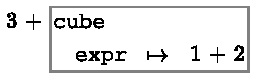
\includegraphics{src/image/gen.pdf}
  \end{center}
  \caption{Program fragment using a \keyword{cube} node, which hasn't been defined.}
  \label{fig-general}
\end{figure}

As seen in Figure \ref{fig-general}, \Meta's implementation does a good job of drawing attention to nodes that aren't handled properly and thus need attention, but it may be overly jarring when used within the context of an otherwise valid expression. Therefore, there may be a role for a less-complete reduction which shows an indication that something is amiss, plus any properly-defined children, in a less obtrusive way.


%
% Editing
%
\section{Editing}
The \Meta\ editor assembles the components described in the previous sections, along with a GUI shell. Each program is displayed in a separate window within a single process. When a grammar is used in the rendering of a program, changes to the grammar are reflected in the program's display immediately. Grammars and other kind of programs are presented and edited in the same way, the only difference being that a different sequence of reductions is applied. Neither the UI nor the programs themselves currently provide any way to specify the reductions that are to be applied to a particular program; it's up to the user to do that when invoking the editor.

An editor window (see Figure\ \ref{fig-editor}) shows a program in a scrollable panel, accompanied by some additional information about the selected node, if any. Actions to edit the program are available in the menus, or via keystrokes.

\begin{figure}[ht]
  \todo{better screenshot?}
  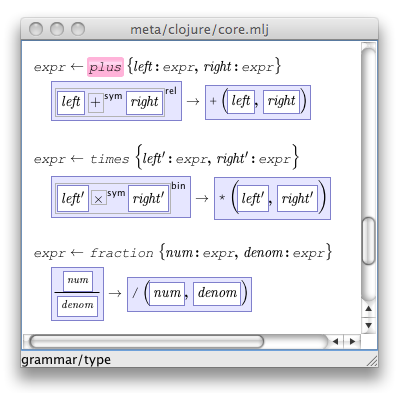
\includegraphics[scale=0.60]{src/image/editor.png}
  \caption{\label{fig-editor} The Meta editor, showing a portion of the grammar for the core language. Part of the definition of the \keyword{plus} node type is selected.}
\end{figure}


\subsection{Rendering Pipeline}
To convert a program into \keyword{view} nodes for rendering, the editor applies a series of reductions in turn, as diagrammed in Figure~\ref{fig-pipeline}. Some of the reductions are baked into the platform, while others are compiled on the fly from the grammars that are specified when the editor is invoked. 

\begin{figure}[ht]
  \todo{draw something; graphviz?}

  \emp{source} : $S$ $\to$ (insert missing nodes) $\to$ $S$ + \keyword{expr/missing} $\to$ (reduce names to expr) $\to$ $S$ + \keyword{expr} $\to$ (meta-reduce source expr nodes [grammars only]) $\to$ (reduce via grammar) $\to$ \keyword{expr} + unreduced nodes $\to$ (reduce un-reduced nodes) $\to$ \keyword{expr} $\to$ (expr-to-view reduction) $\to$ \keyword{view} $\to$ (renderer)

  \caption{Reductions in the rendering pipeline.}
  \label{fig-pipeline} 
\end{figure}

The editor itself takes charge of executing the reductions, keeping track of how the final \keyword{view} nodes were derived from the source program. Thus the end product of the rendering pipeline is a target program in the \keyword{view} language, plus a map identifying the target program node that arose from each source program node. Because a source program node often reduces to a sub-tree rather than a single node, not every target program node is identified with a source; only the root of each sub-tree needs to be tracked. The editor uses this tracking of nodes to let the user interact with the nodes of the \emp{source} program, even though what's actually being rendered is the target program, many layers of reduction removed.

%When it's desirable to keep track of what source node gave rise to a given target node, the reduction can record the labels of each pair of source and target node, forming a kind of mapping between the parallel trees. 
\temp{For this to work, the reduction function needs to operate strictly on the single node it's given, and not reach into any child node. This in turn places some constraints on the way the source program is constructed: each node (along with any environment) must bear sufficient information to identify the correct reduction.}

\subsection{Identifying Nodes by Position}
Once the target program is produced, along with the mapping of origins, the editor can construct a correspondence between source nodes and view-space. Because each target node is identified with a rectangular area of the view, and because each source node is identified with a root target node, the editor can identify the boundary of the visual representation of each source program node. Somewhat more abstractly, the visual arrangement of source nodes can be gleaned, allowing the editor to identify the visible children of each source node, and the order that they appear in the concrete syntax. Based on this information, the editor defines certain relations between source nodes.

The \emp{parent} node is simply the parent in the usual sense. The editor assumes that every ancestor of every visible node is itself visible. Only the root node has no parent.

The \emp{visible children} of a node are the subset of the node's children for which there is some \keyword{view} node, ordered by their visual position. That is, the visible children do not include any child nodes which were ignored by the presentation reduction, and the otherwise unordered children of a map-valued node are ordered according to how they appear in the visual representation of the node. The order is from left to right (sequences) and top to bottom (sections). The children of a \keyword{subscript} node are ordered as follows: nucleus, superscript, subscript.

The \emp{visible siblings} of a node are the visible children of the node's parent. The \emp{next} sibling is defined in the obvious way for all nodes which are not the last visible child of their parent. The \emp{previous} sibling is similarly defined (except for the first visible child). An example of each of these relationships is diagrammed in Figures \ref{fig-position} and \ref{fig-position-tree}.

\begin{figure}
  \todo{annotate}
  
  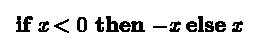
\includegraphics{src/image/position.pdf}
  \caption{Relative node positions, syntax view.}
  \label{fig-position}
\end{figure}

\begin{figure}
  \todo{re-draw as an actual tree}
  
  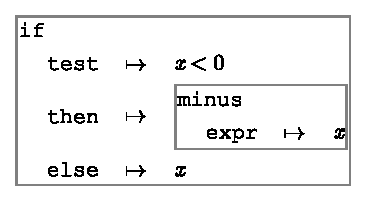
\includegraphics{src/image/position-gen.pdf}
  \caption{Relative node positions, tree view.}
  \label{fig-position-tree}
\end{figure}

\subsection{Selection}
One of the main tasks of the editor is to make the structure of the program visible to the programmer. By rendering the nodes of the program in a rich, familiar notation enhances readability but may not always make the structure of nodes very clear. In order to make a change to the AST, the programmer needs to be aware of this structure. The editor's UI for selection facilitates this awareness by visually emphasizing the relationship between a single selected node and its children, and by providing a way to move between nodes that is defined in terms of the source AST. Thus the structure becomes visible once it is salient, but is left somewhat implicit or even obscured otherwise.

Unlike a text editor, where the typical unit of selection is a character position (i.e. the lowest level of the program text), in \Meta\ the selection identifies a single source-program node which can be at any level of the source tree. A new node can be selected by clicking anywhere in the view. The new selection node is the deepest node whose boundary encloses the clicked location. Once a selection has been established, a new node can be selected by invoking an action to move the selection to a neighboring node using the notion of relative position defined in the previous section. Currently there are actions to select the parent, next or previous sibling, or the first visible child.

%The selection indicator is drawn as a distinctly-colored, slightly rounded rectangle filling in the boundary of the selected node. The boundaries of the visible children are not filled, thus visually emphasizing the relationship between the node and its children. This also means that the filled region corresponds with the region of the display that can be clicked to select that particular node. 

The selected node is the target of all editing operations.

Identifying program elements this way effectively exposes the tree structure of the program to the programmer in a tangible way. requires the programmer to think about the program in terms of its tree structure, so whether or not they feel natural or are easy to understand represents one test of the overall concept of editing the AST.


\subsection{Edit Actions}
The current prototype provides only basic editing operations; to demonstrate a truly usable system would involve more investment in making common operations intuitive and efficient. Edit actions may be invoked through menus or keystrokes. There are just two primitive operations:

\emp{Delete} removes the selected node from its parent. If the parent is a map, it will no longer have any value for the attribute that was occupied by the selected node. If a sequence, the node is removed and any following children move to smaller indices. Note that a simple delete removes an entire subtree, not just the selected node itself.

\emp{Insert} adds a new node as a child of the selected node with a particular attribute name or index. If the selected node is a map, any previous child with the same attribute name is replaced. If a sequence, the new child pushes any existing children to the right.

All other edits are composed out of these operations:

\emp{Replace} deletes the selected node and inserts a new node in the same position.

\emp{Swap with previous} exchanges the places of the selected node and the previous sibling, by a sequence of three replace operations. \emp{Swap with next} is similar.

\emp{Insert parent} Interposes a new node between the selected node and its parent, by deleting the selected node, constructing a new node with it as a child, and then inserting the new node in the same position.

\temp{Change type?}

\temp{Swap with parent?}

\emp{Copy} does not affect the selected node, but saves a reference to it as a separate piece of editor state (the \emp{clipboard}).

\emp{Cut} copies and then deletes the selected node.

\emp{Paste} replaces the selected node with the contents of the clipboard.

When a new node is to be introduced, a simple interface is presented to allow the node's type to be specified. Another UI allows primitive values to be edited.

Before each edit operation, the current source AST and the identity of the selected node are pushed onto a stack of previous states. When the \emp{undo} action is performed, the most recent state is popped from the stack and restored. Because each edit involves $O(\log n)$ nodes, this is efficient enough.

When any editing action changes the source AST, the editor responds by re-reducing the entire program and then redisplays the new reduced view. When a grammar is edited, the grammar itself is re-displayed, and then any reductions that were compiled from it are regenerated and any programs using them are redisplayed as well. This environment allows languages to be redefined dynamically.

%\subsection{Errors \todo{}}

